\documentclass{article}

\usepackage{amsmath}
\usepackage{cleveref}
\usepackage{fullpage}
\usepackage{graphicx}
\usepackage{subcaption}

\newcommand{\ep}{\varepsilon}
\newcommand{\s}{^{[s]}}
\newcommand{\ty}{\tilde{y}_i}
\newcommand{\tX}{\tilde{X}_i}

\begin{document}

\section*{Linear Model}
\subsection*{Problem and General Approach}

Suppose that we are estimating a linear model of the form
\begin{equation}
	\label{eq:lm}
	y = X \beta + \ep,
\end{equation}
where $y$ is a $N\times 1$ vector of observed outputs, $X$ is a $N\times k$ matrix of observed inputs, $\beta$ is a $k\times 1$ vector of slope parameters, and $\ep\sim N(0, \sigma^2 I)$ is a $N\times 1$ vector of error terms. Samples of parameters $\beta | y, X$ and $\sigma | y, X$ can be obtained through application of an MCMC algorithm, given priors on parameters $\beta$ and $\sigma$. Also suppose that $X$ follows some distribution $p(X | \theta_X)$, where $\theta_X$ are parameters of that distribution.

Given a scalar output value $\ty$, our goal is to estimate the distribution of inputs that could have resulted in $\ty$, given by $p(\tX | \ty, y, X, \theta_X)$, where $\ty = \tX \beta + \tilde{\ep}_i$. We'll start by considering $p(\tX | \ty, y, X, \theta_X, \beta, \sigma)$. Notice that
\begin{align}
	\label{eq:conditional-posterior}
	\nonumber
	p(\tX | \ty, y, X, \theta_X, \beta, \sigma) &\propto p(\ty | \tX, y, X, \theta_X, \beta, \sigma) p(\tX | y, X, \theta_X, \beta, \sigma) \\
	&\equiv p(\ty | \tX, \beta, \sigma) p(\tX | \theta_X).
\end{align}
This relationship immediately reveals a general sampling approach for $\tX | \ty, y, X, \theta_X, \beta, \sigma$: $p(\tX | \theta_X)$ acts as the prior and $p(\ty | \tX, \beta, \sigma)$ acts as the likelihood, resulting in the posterior $p(\tX | \ty, y, X, \theta_X, \beta, \sigma)$. Samples of the posterior can be generated by the application of any appropriate MCMC algorithm, such as Metropolis-Hastings (MH) or Hamiltonian Monte Carlo (HMC).

In practice, of course, parameters $\beta$ and $\sigma$ are not known. To address this issue, we can simply integrate those parameters out:
\begin{align}
	p(\tX | \ty, y, X, \theta_X) &= \int p(\tX | \ty, y, X, \theta_X, \beta, \sigma) p(\beta | y, X) p(\sigma | y, X) d\beta d\sigma \\
	&\propto \int p(\ty | \tX, \beta, \sigma) p(\tX | \theta_X) p(\beta | y, X) p(\sigma | y, X) d\beta d\sigma.
\end{align}
This reveals a general sampling approach for $\tX | \ty, y, X, \theta_X$:
\begin{enumerate}
	\item Obtain samples of $\beta | y, X$ and $\sigma | y, X$ through the application of an appropriate MCMC algorithm to estimate \Cref{eq:lm}. This results in samples $\beta\s | y, X$ and $\sigma\s | y, X$, where $s = 1, ..., S$.
	\item For each $s$, generate samples of $\tX | \ty, y, X, \theta_X, \beta\s, \sigma\s$ using \Cref{eq:conditional-posterior}.
	\item Combining samples of $\tX | \ty, y, X, \theta_X, \beta\s, \sigma\s$ across $s = 1, ..., S$ results in samples of $\tX | \ty, y, X, \theta_X$.
\end{enumerate}

The final challenge is to accommodate various distributions for $\tX$. We'll start by illustrating the simple case where $\tX$ follows a multivariate normal distribution. We will then relax that assumption to allow $\tX$ to follow a mixture of multivariate normals, which provides adequate approximation to a wide range of empirical distributions and datasets.

\subsection*{Example: $\tX\sim N(\mu_X, \Sigma_X)$}

We will begin with an example where $\tX$ follows a multivariate normal distribution. For purposes of estimation, we will separate the constant term from variable inputs, resulting in the linear model
\begin{equation}
	y_i = \alpha + X_i \beta + \ep_i,
\end{equation}
where $\alpha$ is a scalar parameter, $\beta$ is a $k\times 1$ parameter vector, and $\ep_i \sim \mbox{iid }N(0, \sigma^2)$. Notice that there are $k+2$ parameters in this model formulation.

For this example, we use population and parameter values shown in \Cref{tab:lm-normal-params}.
\begin{table}
\centering
\begin{tabular}{|c|c|}
	\hline
	\textbf{Parameter} & \textbf{Value} \\ \hline
	$N$ & 100 \\ \hline
	$k$ & 2 \\ \hline
	$\alpha$ & 4 \\ \hline
	$\beta$ & $\begin{bmatrix} -2.5 \\ -1.25 \end{bmatrix}$ \\ \hline
	$\sigma$ & 0.4 \\ \hline
	$\mu_X$ & $\begin{bmatrix} -3 \\ 4\end{bmatrix}$ \\ \hline
	$\Sigma_X$ & $\begin{bmatrix} 4.5 & -0.75 \\ -0.75 & 1.25 \end{bmatrix}$ \\ \hline
\end{tabular}
\caption{Parameter values}
\label{tab:lm-normal-params}
\end{table}
Values of $X_i$ were generated using $X_i \sim \mbox{iid } N(\mu_X, \Sigma_X)$, values of $\ep_i$ were generated using $\ep_i \sim \mbox{iid } N(0, \sigma^2)$, and values of $y$ were generated using $y = X\beta + \ep$. The bivariate density of $X$ is shown in \Cref{fig:lm-normal-X} and the density of $y$ is shown in \Cref{fig:lm-normal-y}; note that particular values of $X$ and $y$ are singled out in red, which we'll return to later.
\begin{figure}
	\centering
	\begin{subfigure}{0.5\linewidth}
		\centering 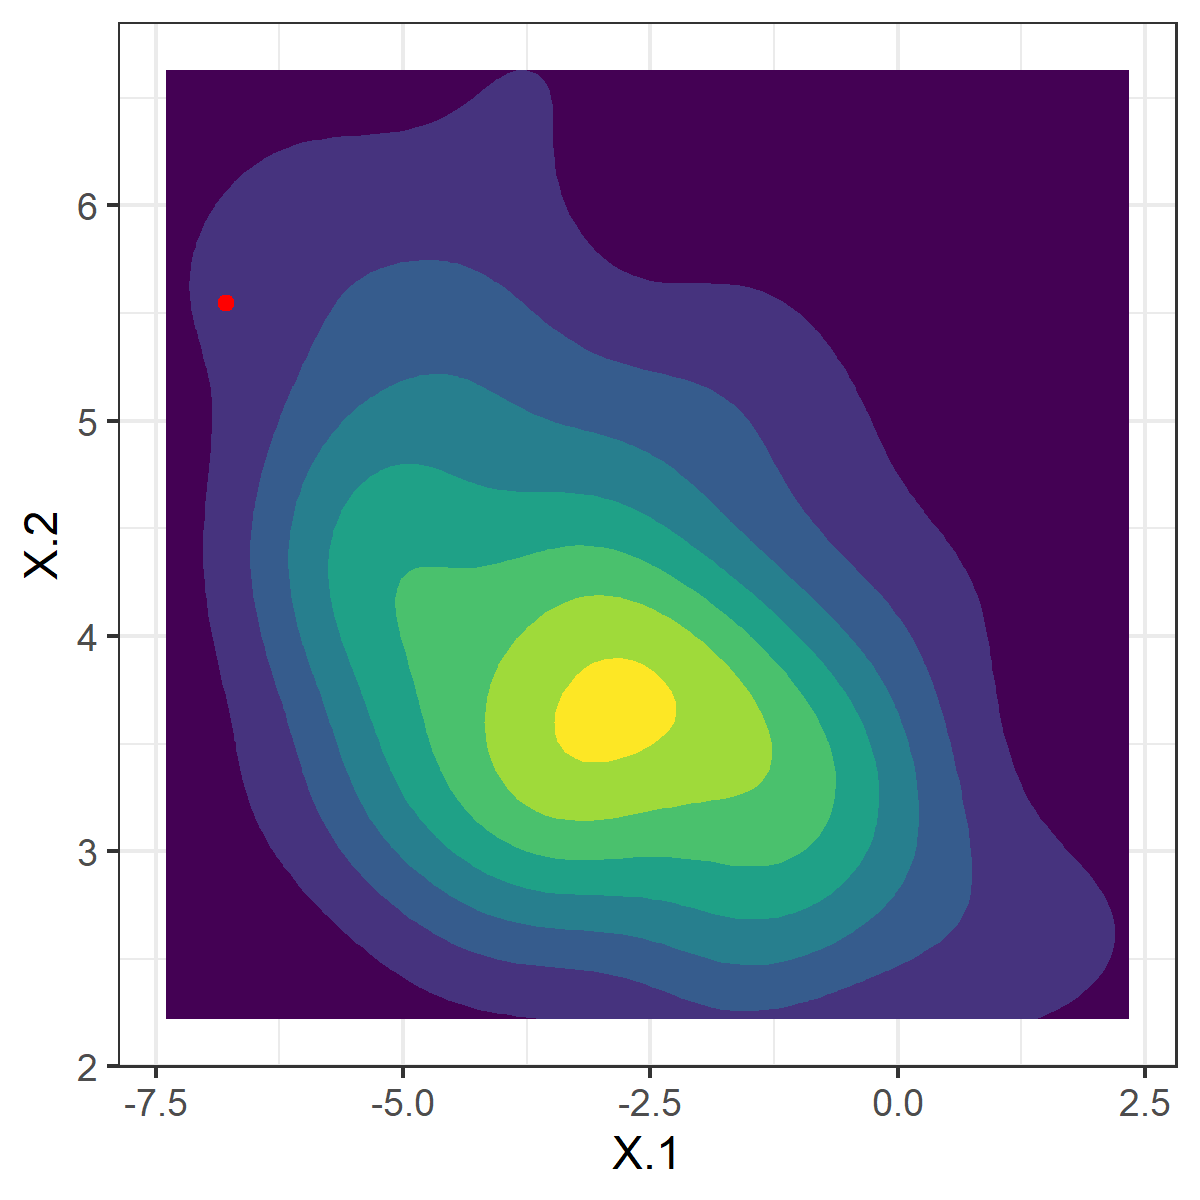
\includegraphics[width=\linewidth]{../examples/lm-normal-fixed/images/density-X.png}
		\caption{Density of $X$}
		\label{fig:lm-normal-X}
	\end{subfigure}%
	\begin{subfigure}{0.5\linewidth}
		\centering 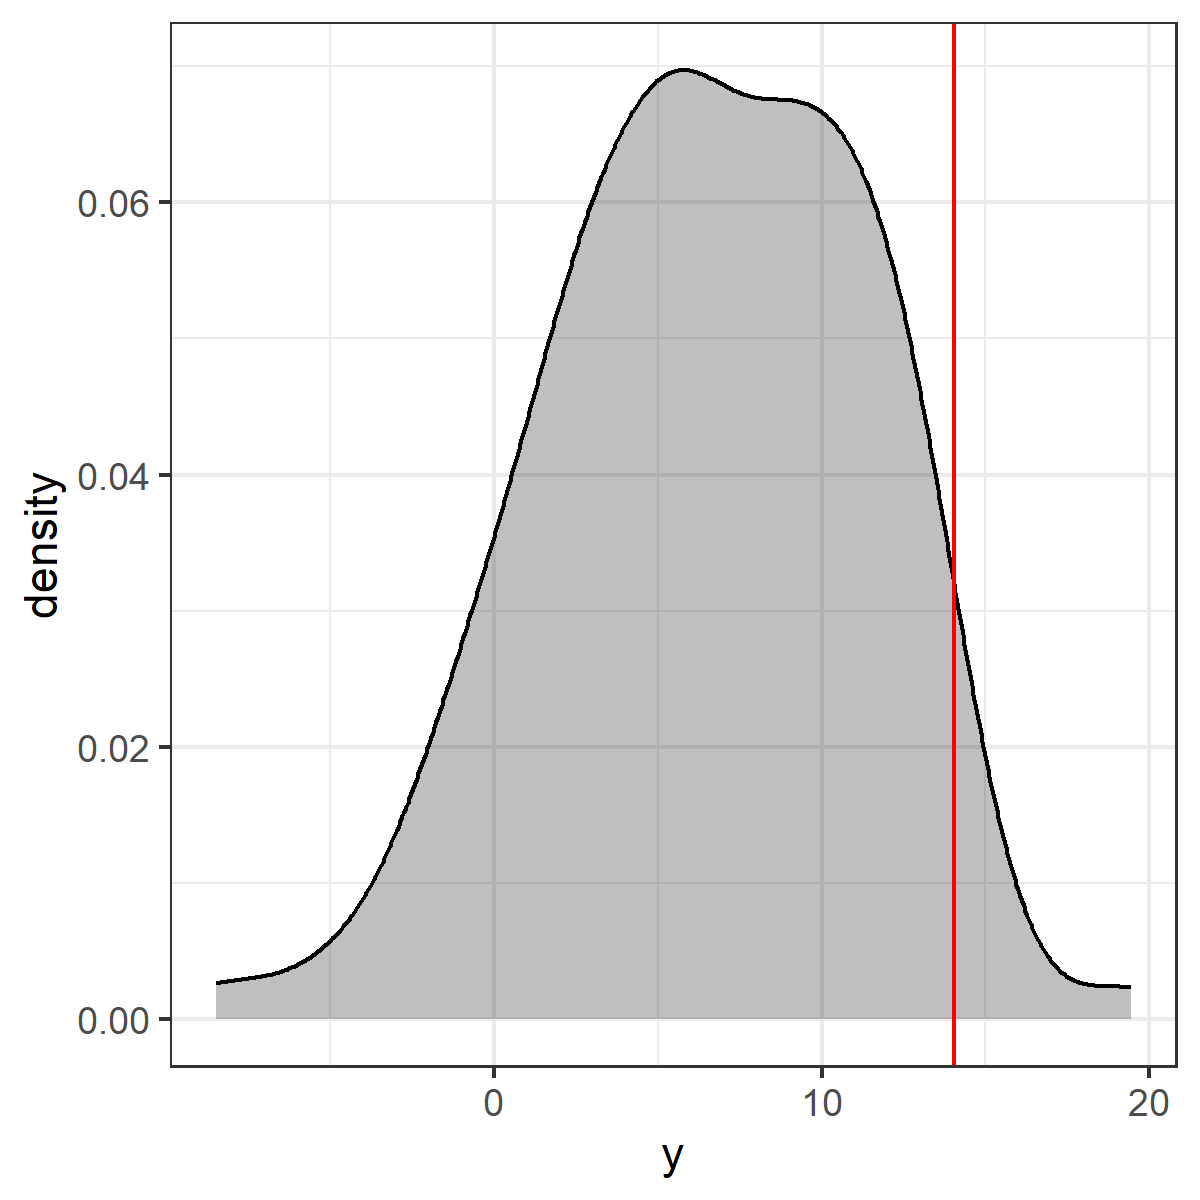
\includegraphics[width=\linewidth]{../examples/lm-normal-fixed/images/density-y.png}
		\caption{Density of $y$}
		\label{fig:lm-normal-y}
	\end{subfigure}
	\caption{Densities of observed data}
	\label{fig:lm-normal-densities}
\end{figure}

Samples of parameters $\alpha, \beta, \sigma | y, X$ were generated using No U-Turn Sampling (NUTS) as implemented in Stan, using priors shown in \Cref{tab:lm-normal-priors}. The sampling procedure used a single chain with 1000 warmup iterations and 1000 sampling iterations, and standard convergence diagnostics were applied. Posterior densities are shown in \Cref{fig:lm-normal-posterior-forward}.
\begin{table}
\centering
\begin{tabular}{|c|c|}
	\hline
	\textbf{Parameter} & \textbf{Prior} \\ \hline
	$\alpha$ & $N(0, 100)$ \\ \hline
	$\beta$ & $N(0, 100I)$ \\ \hline
	$\sigma$ & $\mbox{Cauchy}(0, 1)$ \\ \hline
\end{tabular}
\caption{Parameter priors}
\label{tab:lm-normal-priors}
\end{table}
\begin{figure}
	\centering
	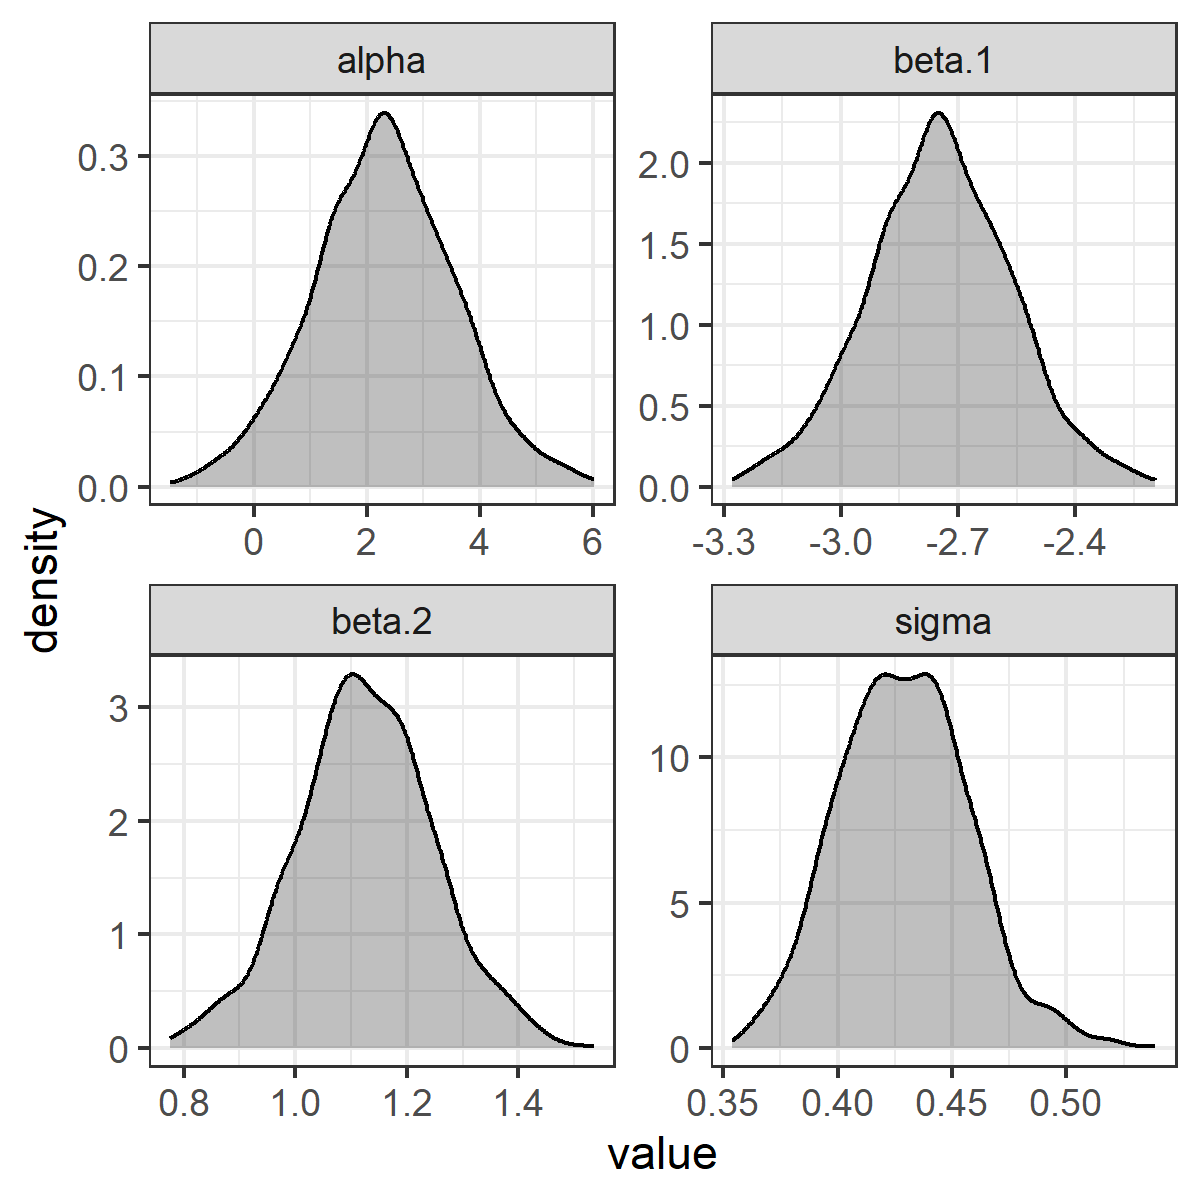
\includegraphics[width=4in]{../examples/lm-normal-fixed/images/density-posterior-forward.png}
	\caption{Parameter posterior densities}
	\label{fig:lm-normal-posterior-forward}
\end{figure}

Next, a particular observation of $X$ and $y$ was singled out to validate the inverse propagation procedure. Specifically, we used an observation of $\tX\approx \begin{bmatrix} -6.79 & 5.55 \end{bmatrix}'$ and $\ty = \alpha + \tX \beta \approx 14.04$, shown in red in \Cref{fig:lm-normal-densities}. The sampling procedure laid out in the General Approach section was used to generate samples of $\tX | \ty, y, X, \theta_X$ using NUTS, and standard convergence checks were again applied. The resulting posterior distribution of $\tX$ and actual value of $X$ are shown in \Cref{fig:lm-normal-posterior-inverse}.
\begin{figure}
	\centering
	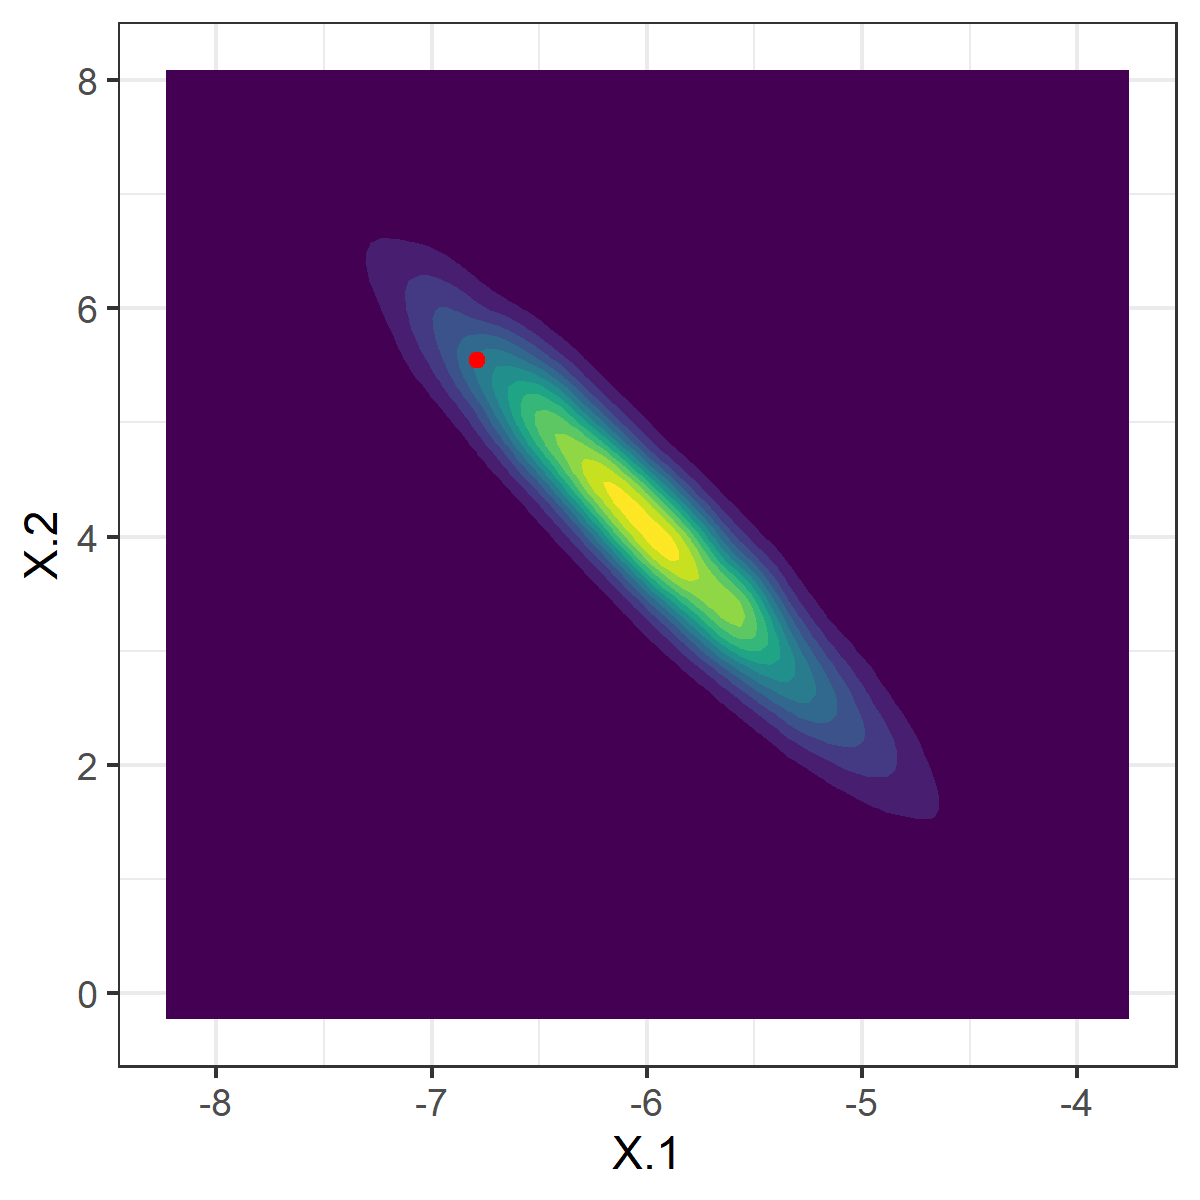
\includegraphics[width=4in]{../examples/lm-normal-fixed/images/density-posterior-inverse.png}
	\caption{Posterior density of $\tX$}
	\label{fig:lm-normal-posterior-inverse}
\end{figure}

To analyze this fit, we've recreated \Cref{fig:lm-normal-posterior-inverse} with two additional lines in \Cref{fig:lm-normal-posterior-inverse-pca}.
\begin{figure}
	\centering
	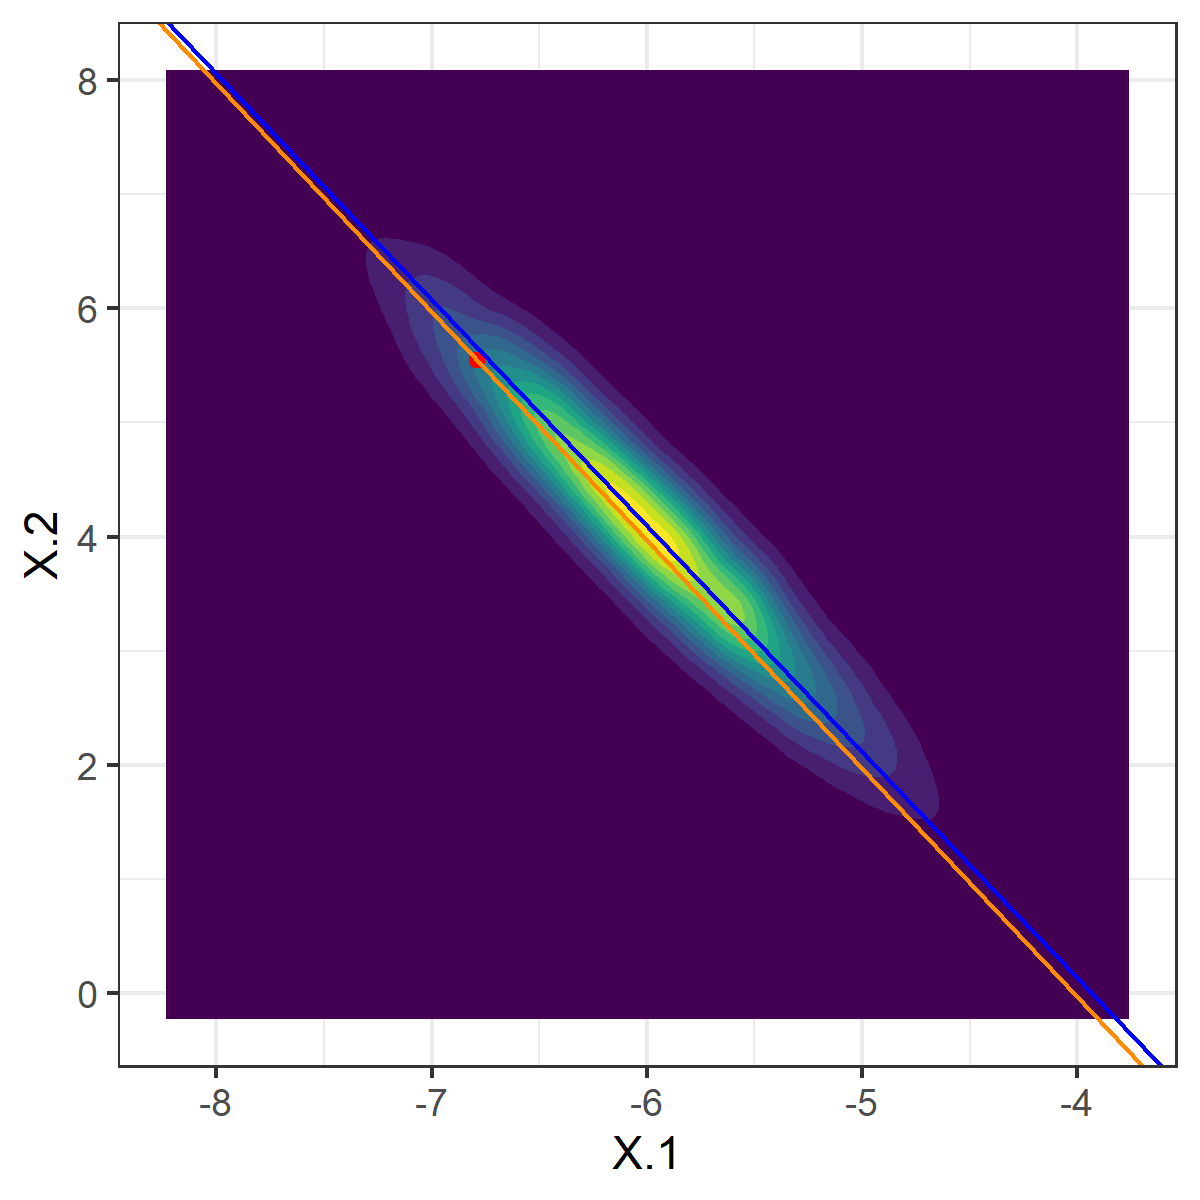
\includegraphics[width=4in]{../examples/lm-normal-fixed/images/density-posterior-inverse-pca.png}
	\caption{Posterior density of $\tX$ with solution line and PCA}
	\label{fig:lm-normal-posterior-inverse-pca}
\end{figure}
The orange line represents all values of $X_i$ such that the equation $\ty = X_i \beta$ is satisfied. Since $\ty$ was generated without a random error component, the true value of $\tX$ is necessarily on this line. Values of $X_i$ not on the orange line must have some non-zero error component in order for $\ty = X_i \beta + \ep_i$ to be satisfied. The blue line shows the first principal component of the posterior sample of $\tX$.

\subsection*{Example: $\tX$ Follows a Mixture of Normals}

In this example, we make all the same assumptions as the previous example, except we generalize to the case where $\tX$ follows a mixture of normal distributions. That is, there are mixing probabilities $m_1, ..., m_C$ with $\sum_c m_c = 1$ such that
\begin{equation}
	p(X | \theta_X) = \sum_c m_c p(X | \mu_c, \Sigma_c),
\end{equation}
where $p(X | \mu_c, \Sigma_c)$ is a multivariate normal distribution with known mean $\mu_c$ and variance $\Sigma_c$. As before, we can note that 
\begin{align}
	\label{eq:conditional-posterior}
	\nonumber
	p(\tX | \ty, y, X, \theta_X, \beta, \sigma) &\propto p(\ty | \tX, \beta, \sigma) p(\tX | \theta_X) \\
	& \equiv p(\ty | \tX, \beta, \sigma) \sum_c m_c p(\tX | \mu_c, \Sigma_c)
\end{align}

\end{document}